\section{Test: Vestas Turbine Simulator} \label{sec:test_vts}
This section contains the results of the test of the controller in Vestas Turbine Simulator (VTS). It is split into two sections. In the first section the LQI controller is compared with the FLC PI controller without FATD and with the FLC PI controller detuned to reduce the fore-aft negative damping phenomena. In the second section the LQI controller performance at 12 m/s and 26 m/s wind speed is shown with the LQI controller parameters recalculated at said operating points. The controller performance is compared across 12, 16 and 26 m/s wind speeds.

\subsection{Part 1}


\begin{figure}[ht]
	\centering
	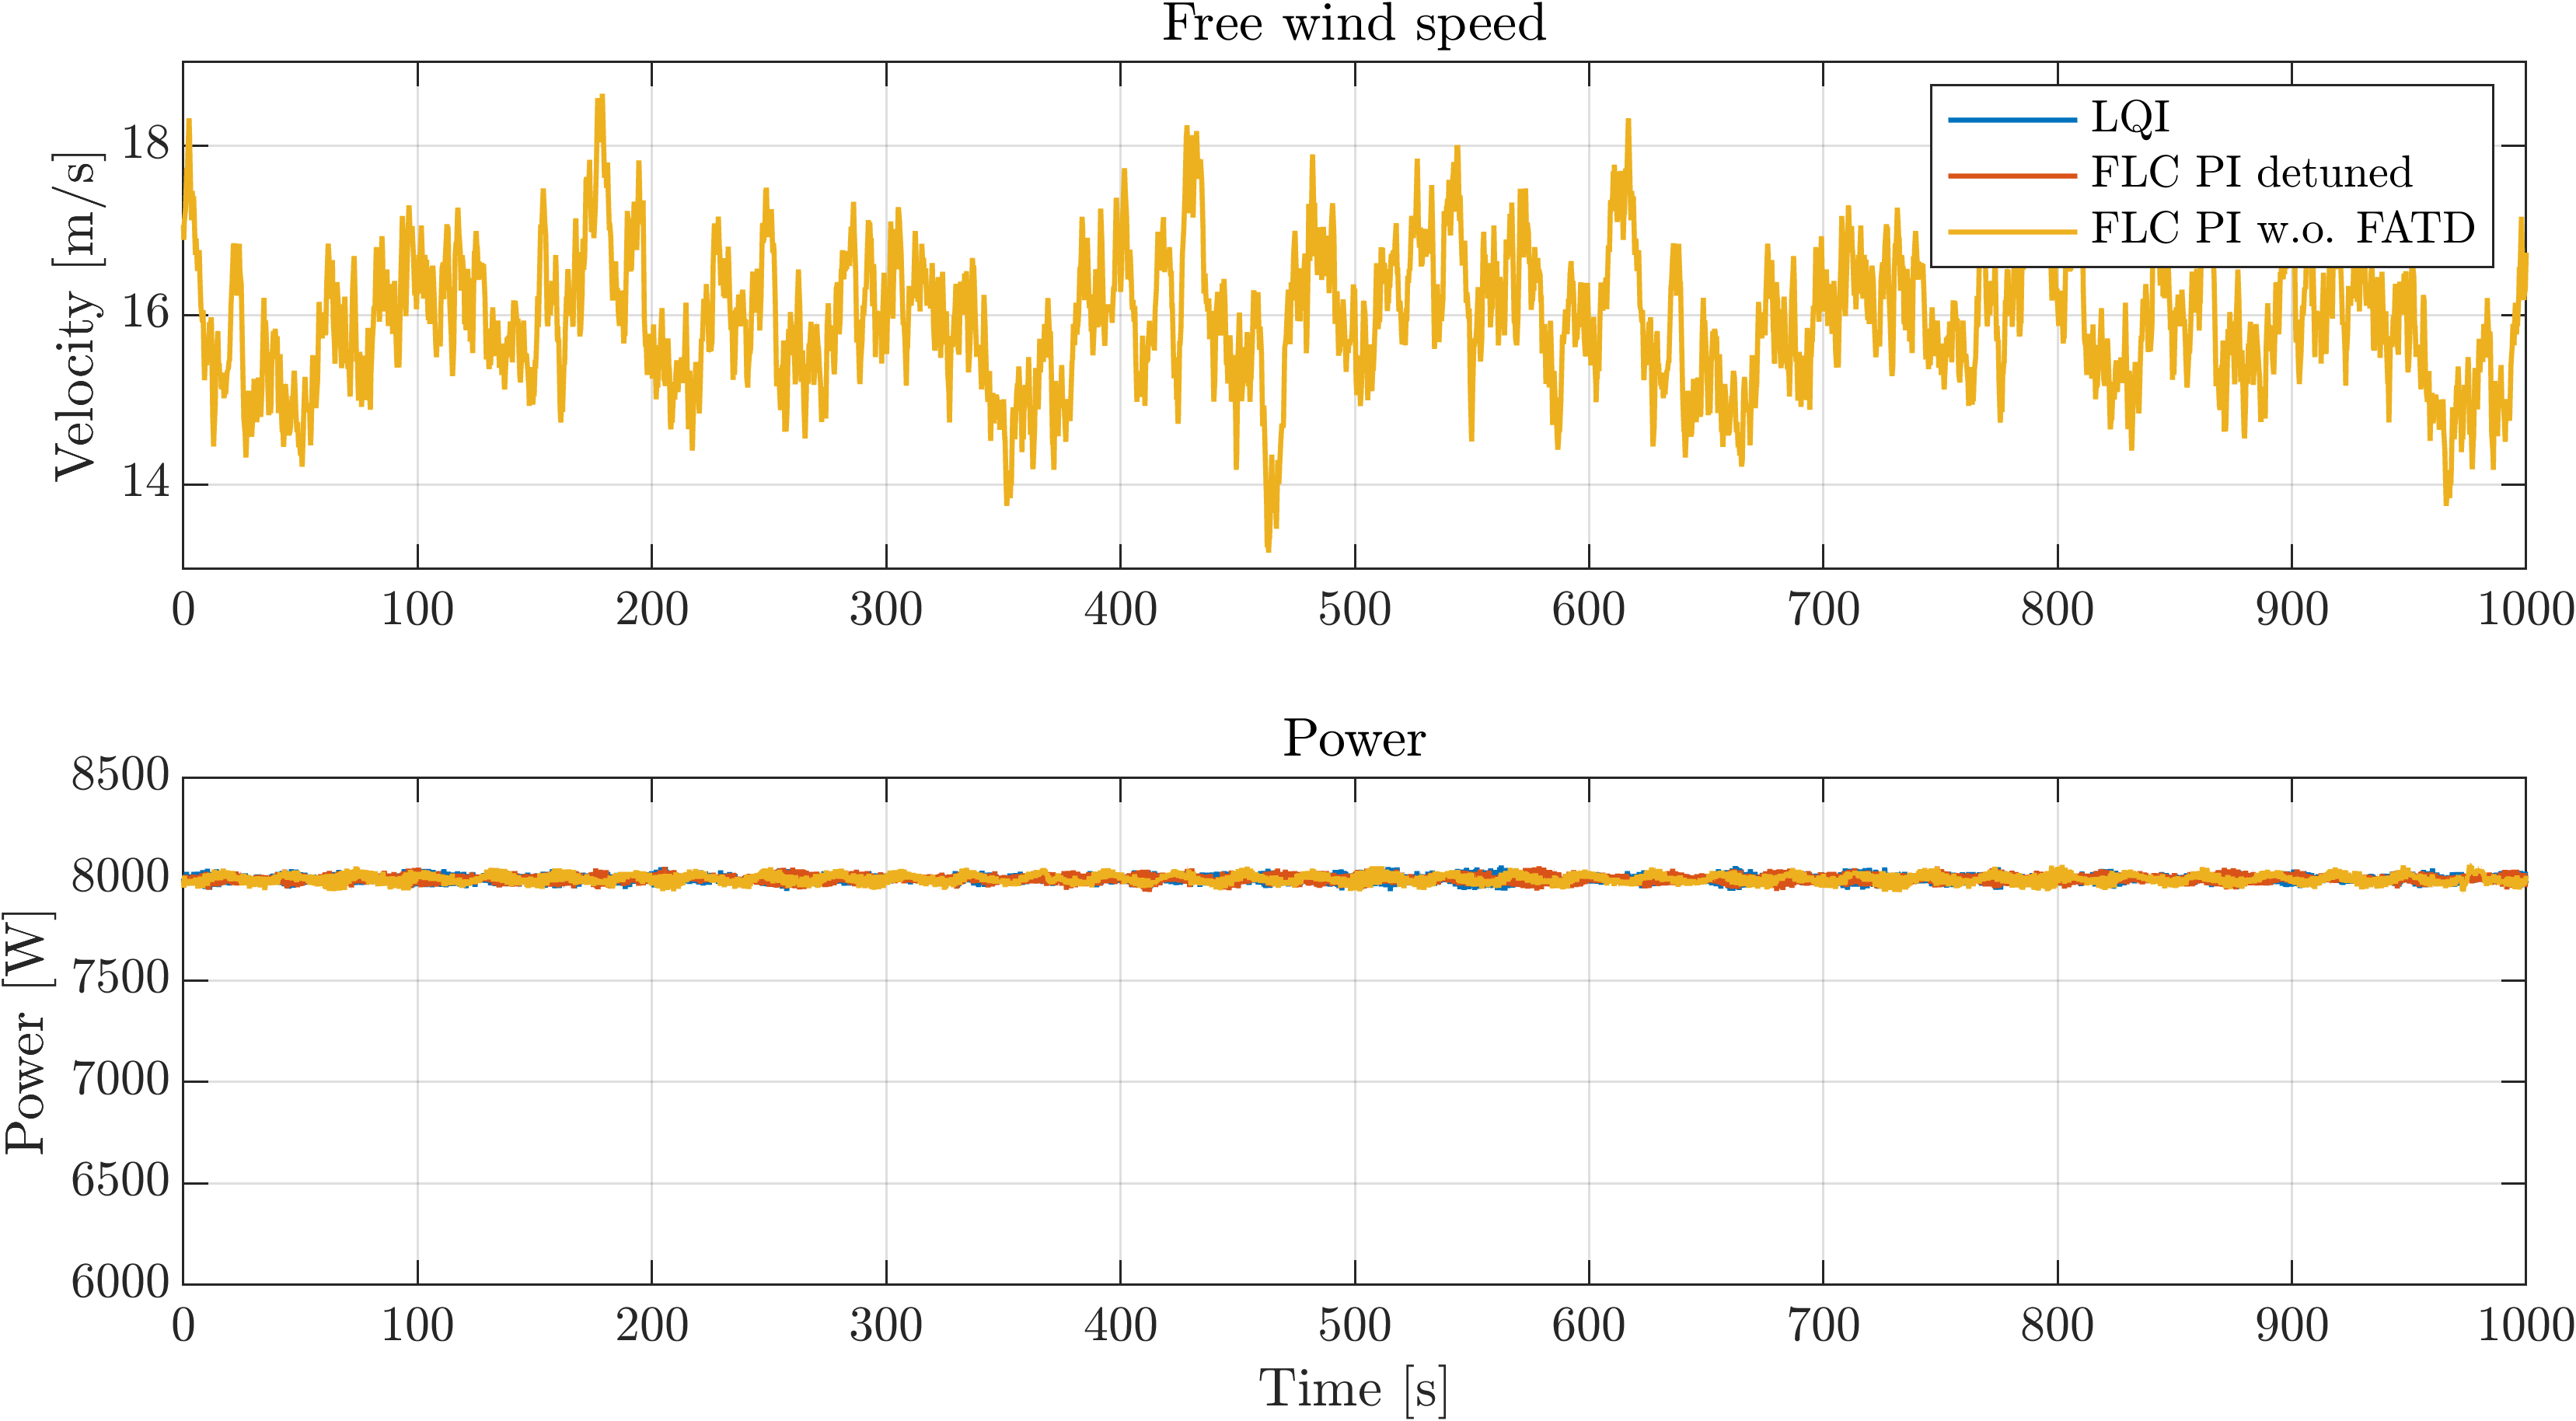
\includegraphics[width=0.7\linewidth]{Graphics/TestResults/VTSplotting/1_wind_pow.png}
	\caption{VTS simulation results.}
	\label{fig:vts_1_wind_pow}
\end{figure}

\begin{figure}[ht]
	\centering
	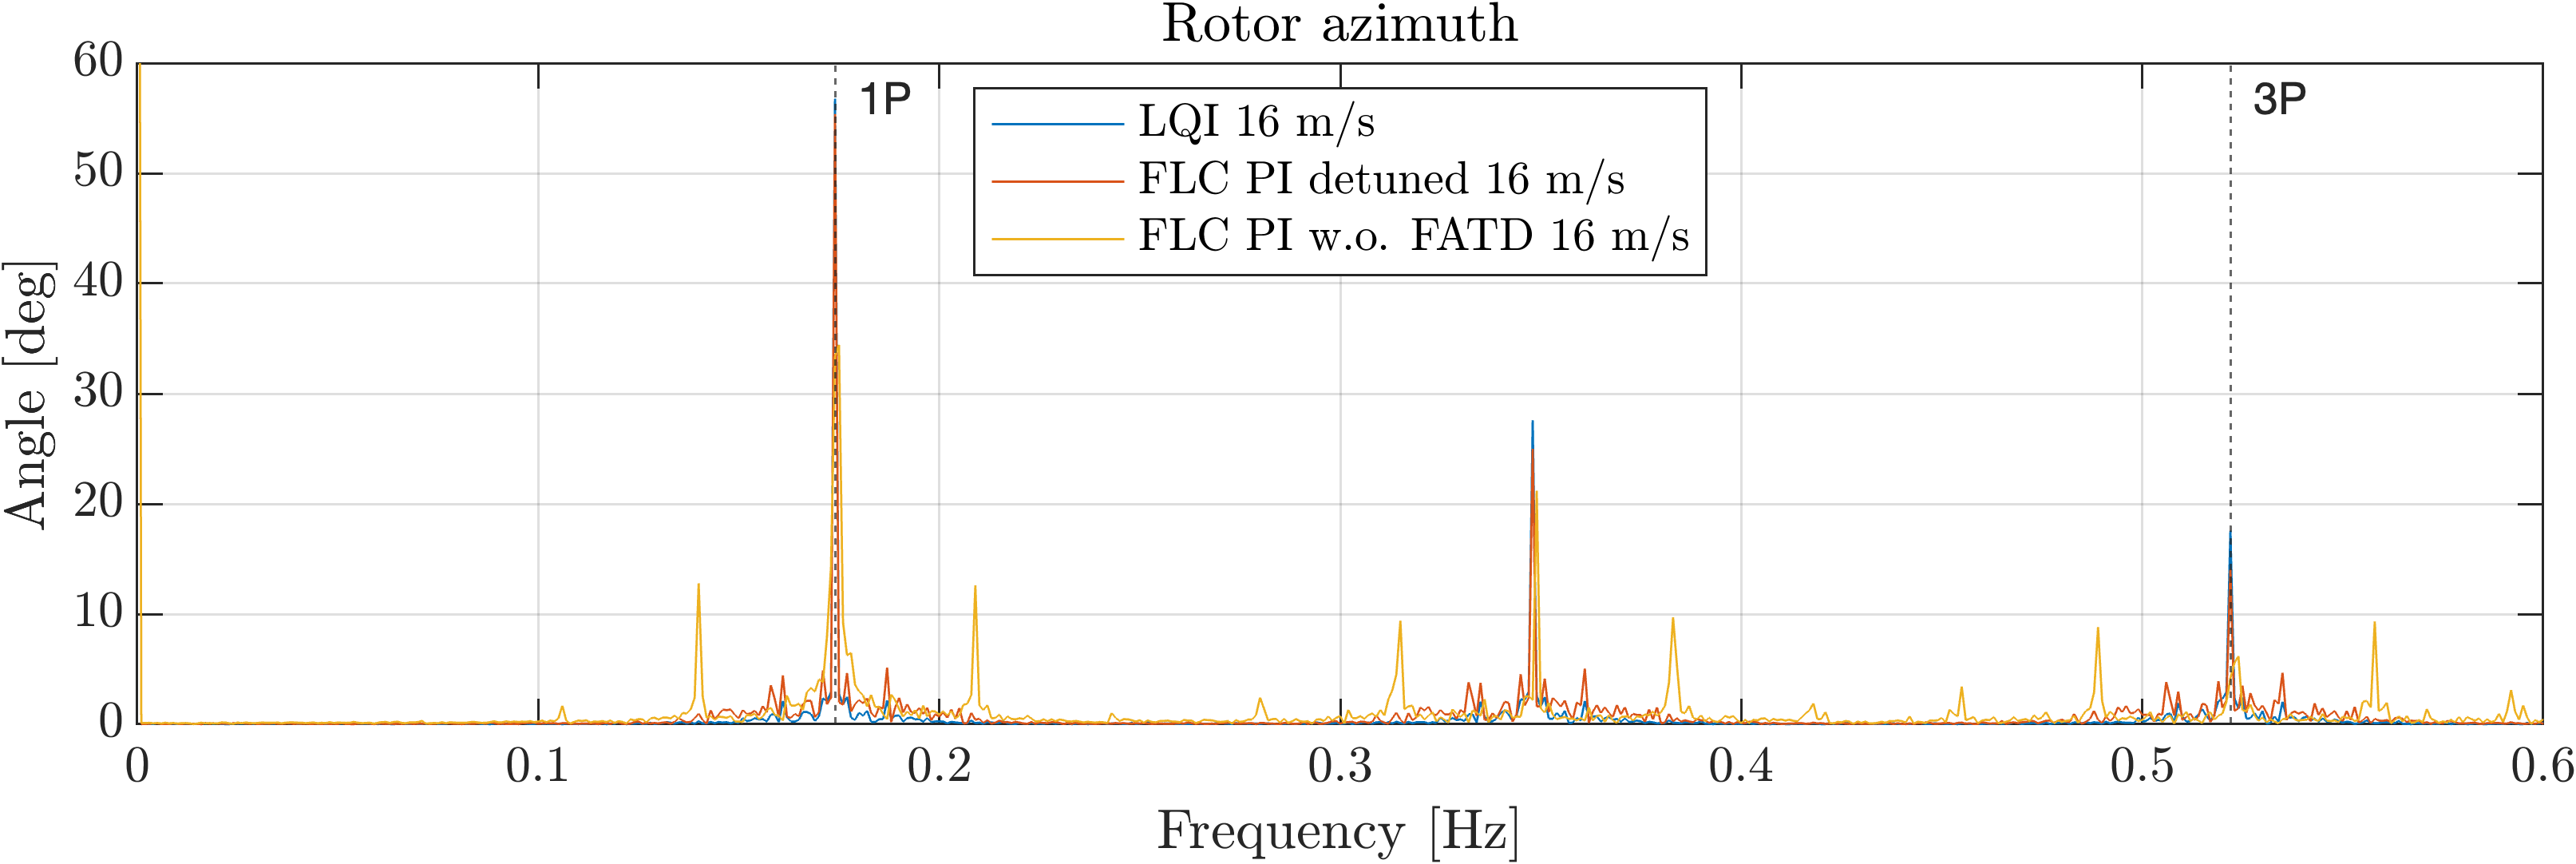
\includegraphics[width=0.7\linewidth]{Graphics/TestResults/VTSplotting/2_fftazi.png}
	\caption{VTS simulation results.}
	\label{fig:vts_2_fftazi}
\end{figure}

\begin{figure}[ht]
	\centering
	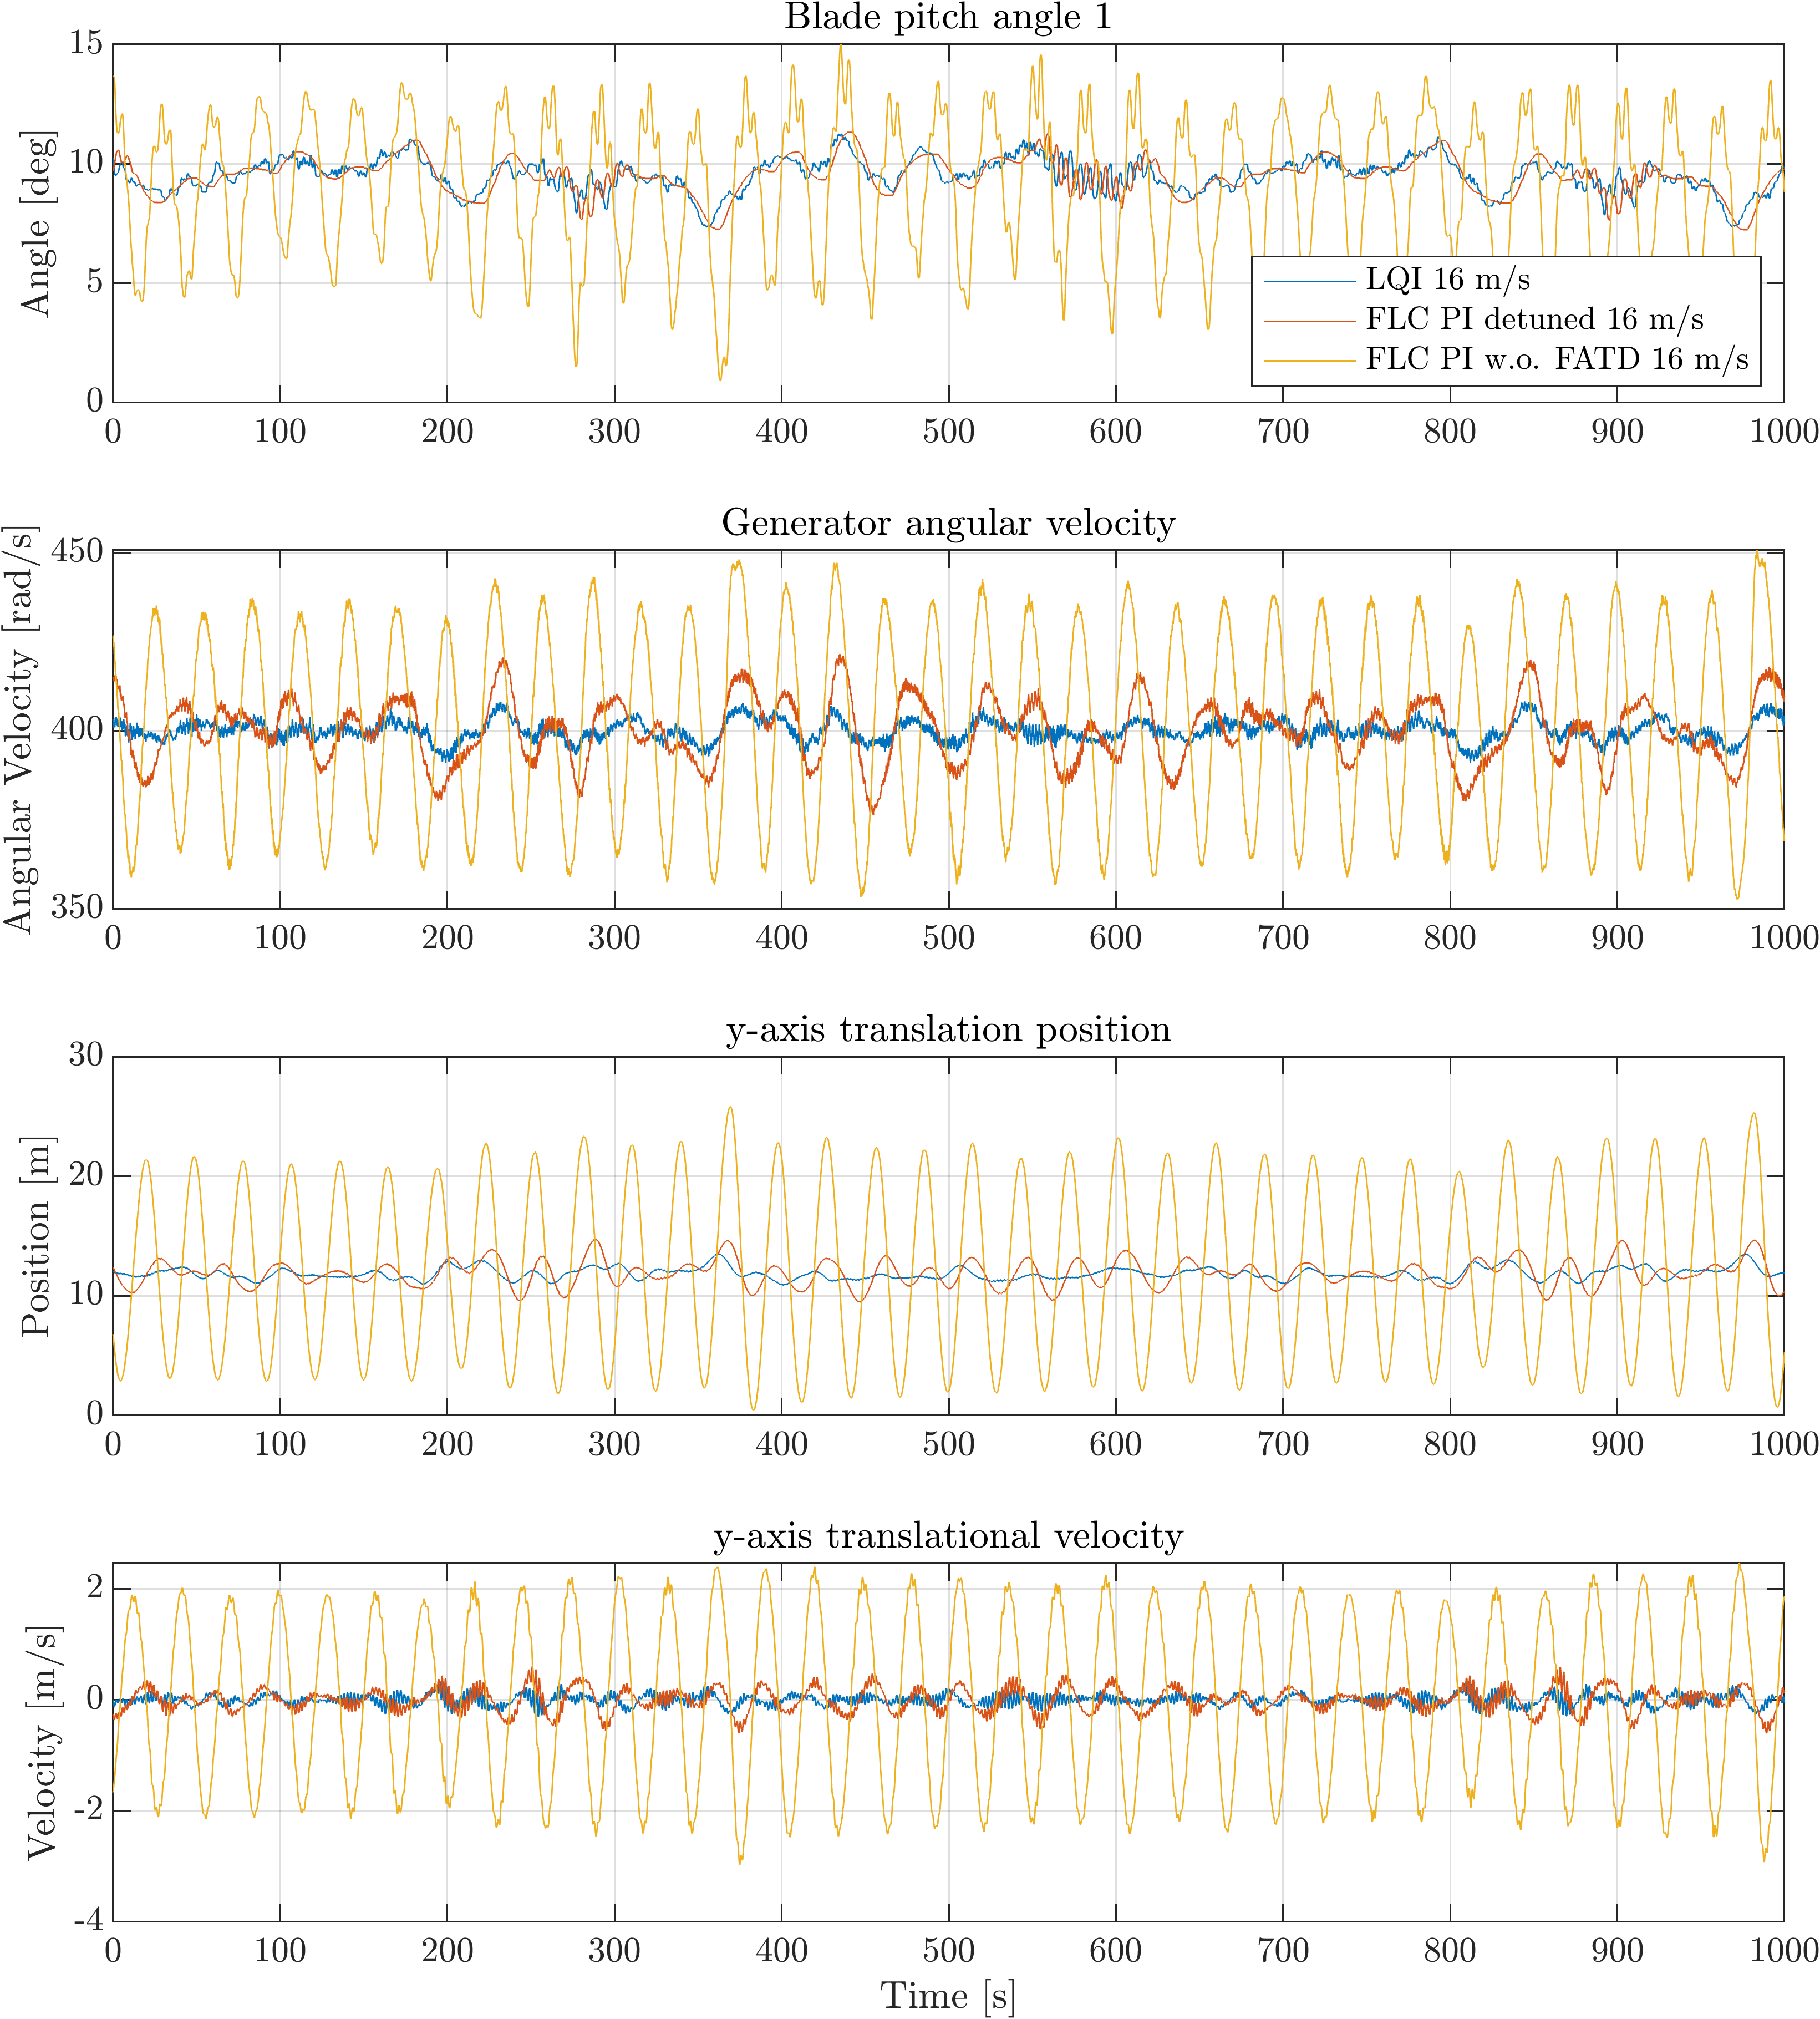
\includegraphics[width=0.7\linewidth]{Graphics/TestResults/VTSplotting/3_th_w_py_vy.png}
	\caption{VTS simulation results.}
	\label{fig:vts_3_th_w_py_vy}
\end{figure}

\begin{figure}[ht]
	\centering
	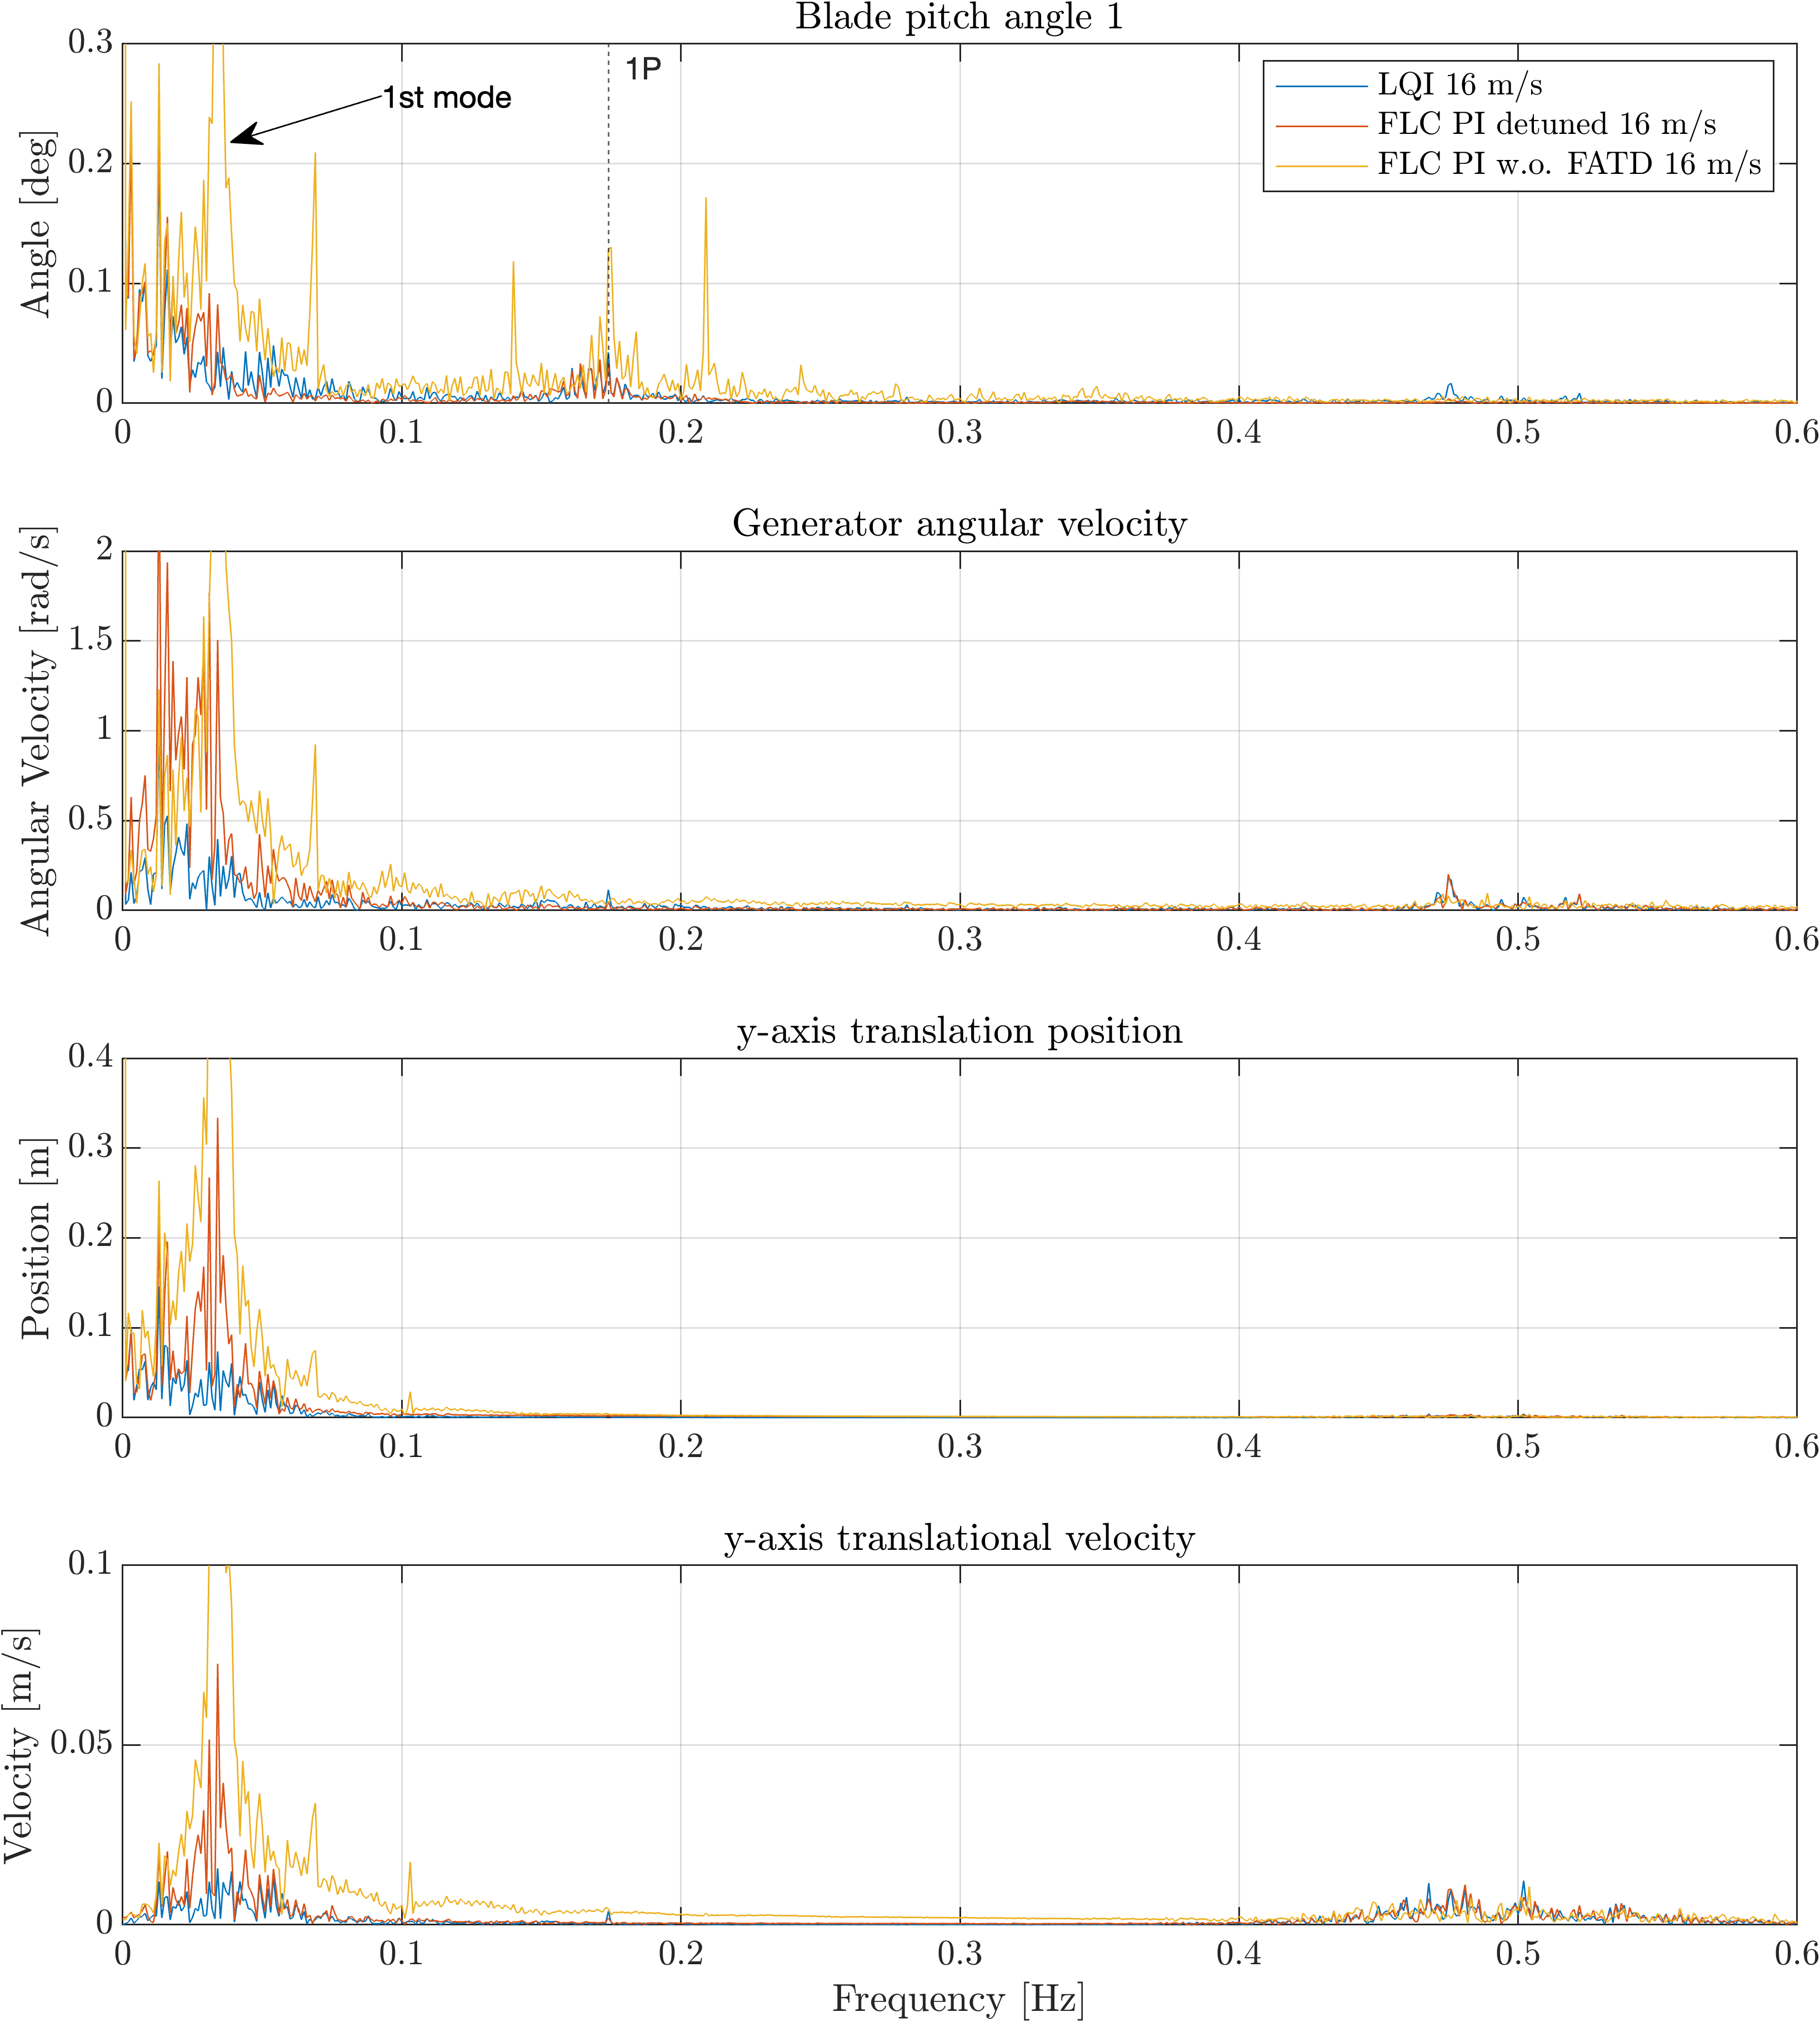
\includegraphics[width=0.7\linewidth]{Graphics/TestResults/VTSplotting/4_fft_th_w_py_vy.png}
	\caption{VTS simulation results.}
	\label{fig:vts_4_fft_th_w_py_vy}
\end{figure}

\begin{figure}[ht]
	\centering
	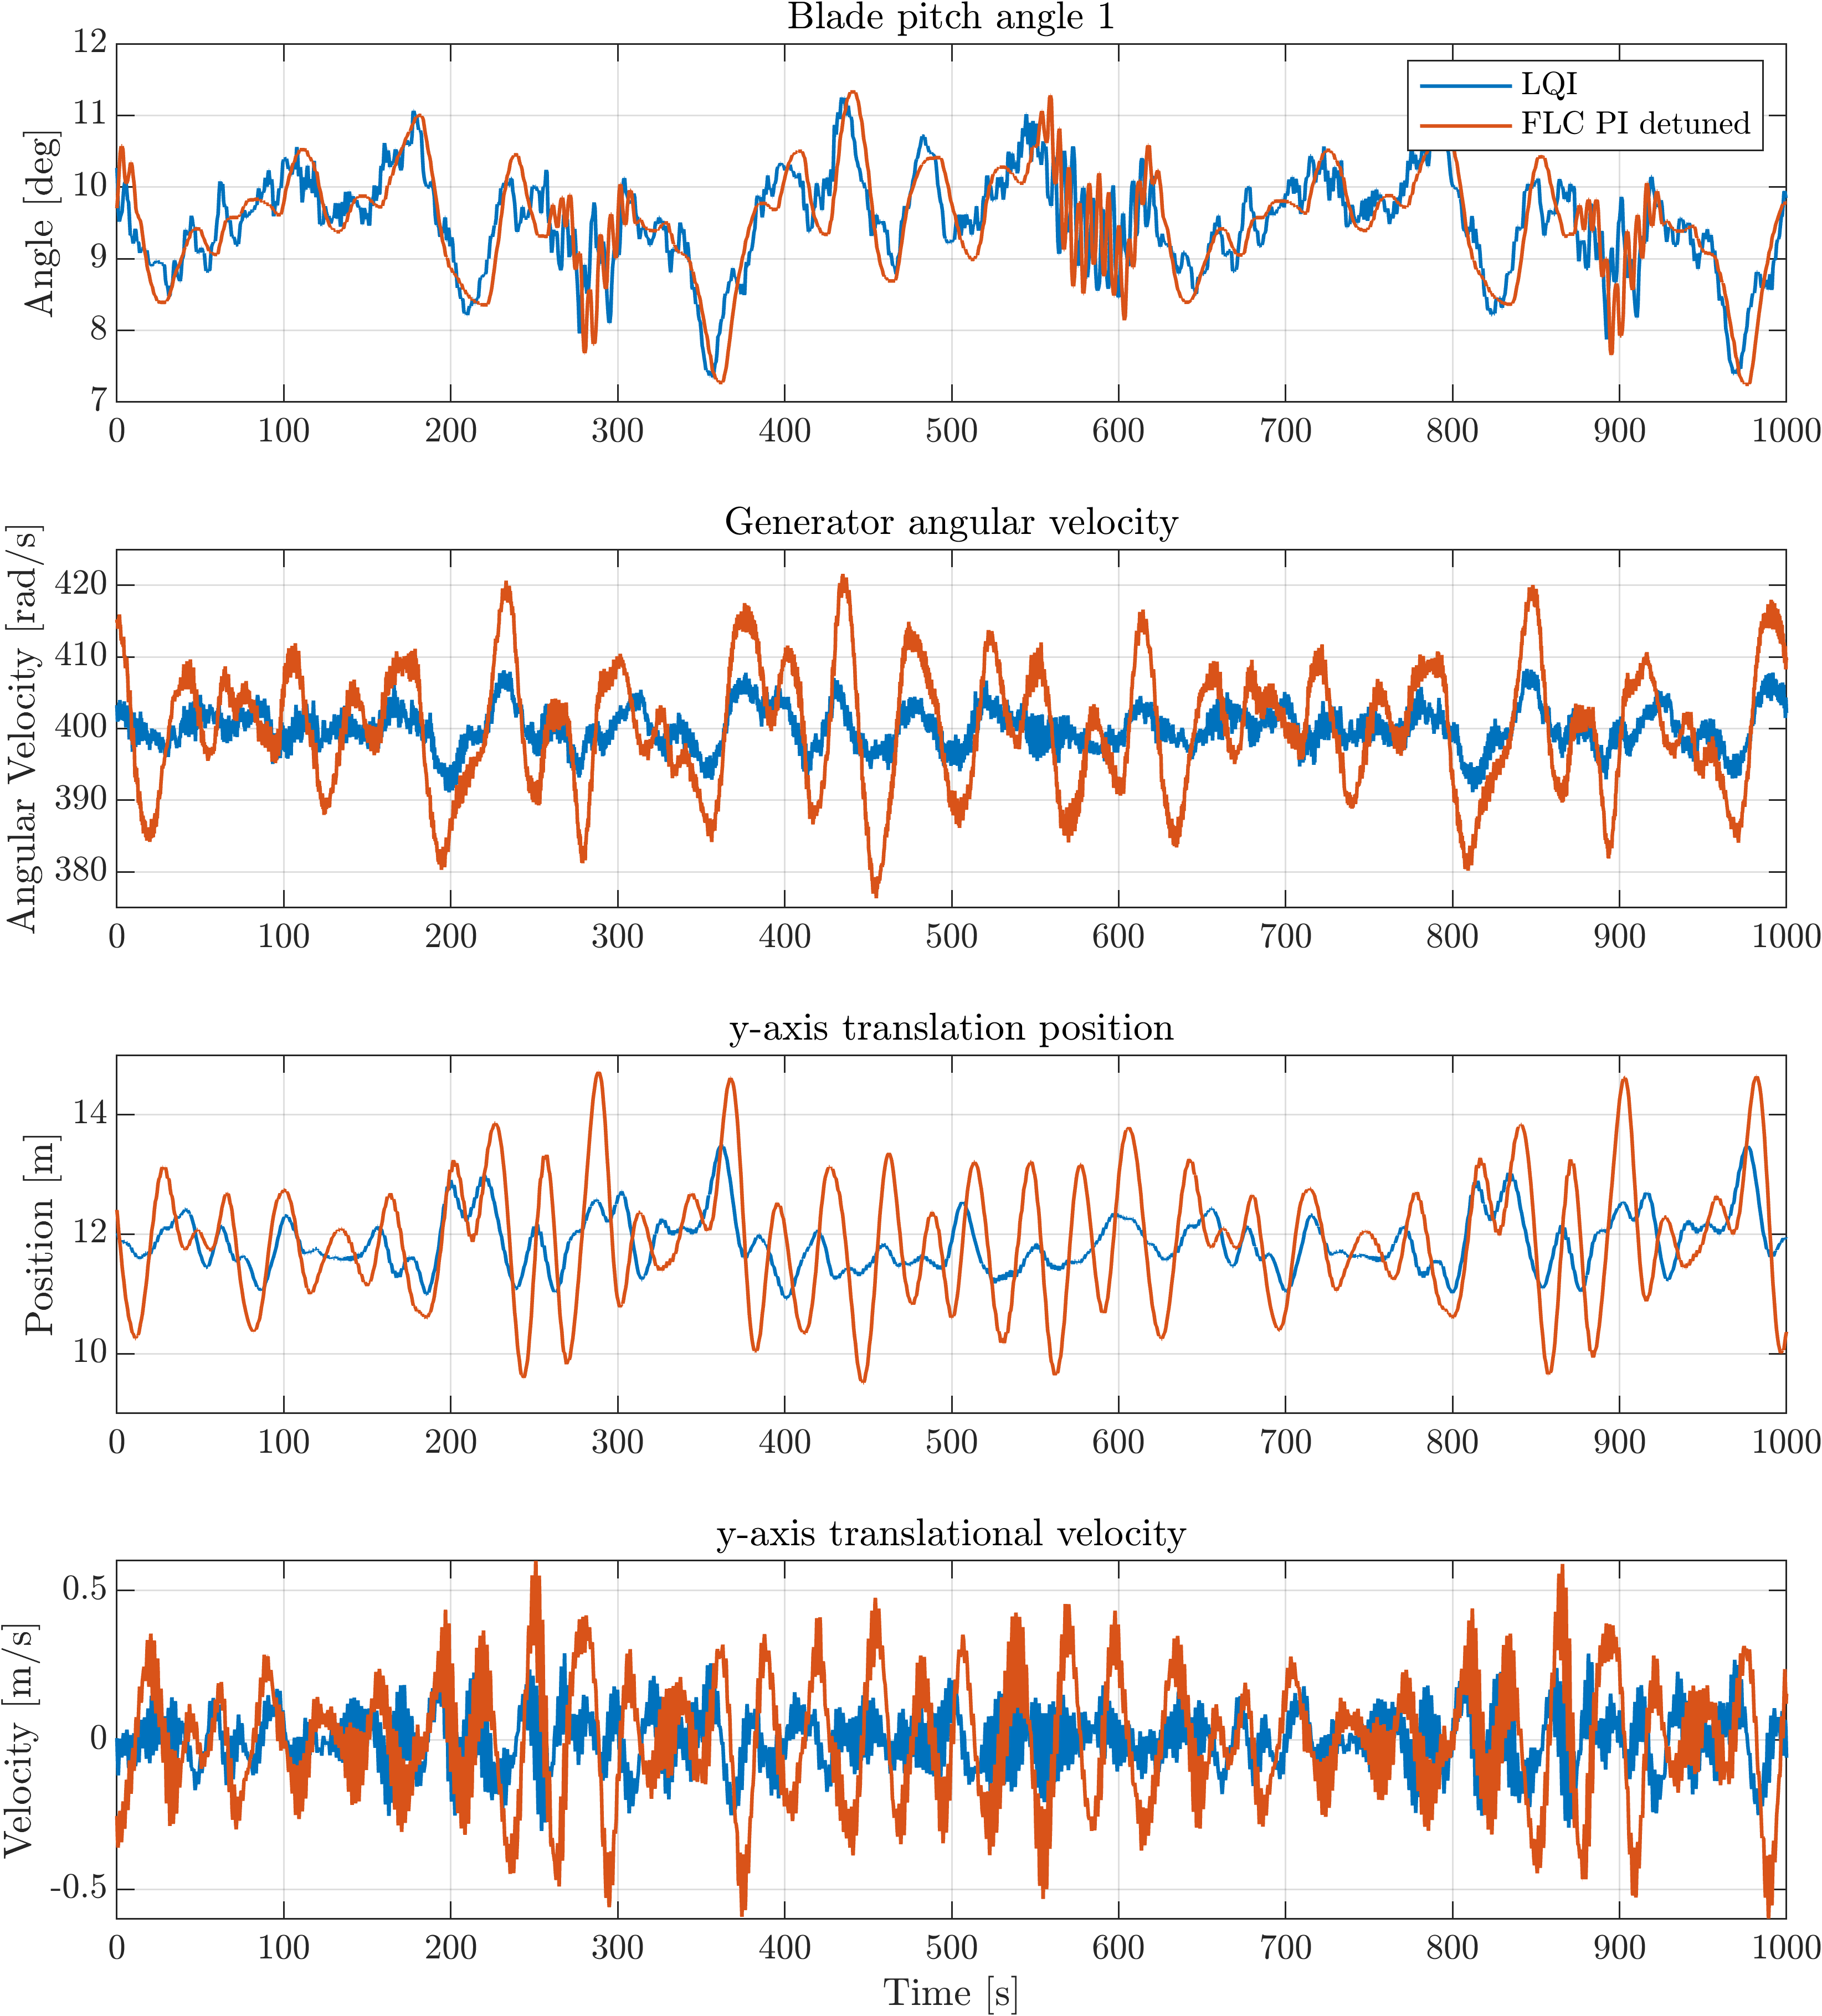
\includegraphics[width=0.7\linewidth]{Graphics/TestResults/VTSplotting/10_th_w_py_vy.png}
	\caption{VTS simulation results.}
	\label{fig:vts_10_th_w_py_vy}
\end{figure}

\begin{figure}[ht]
	\centering
	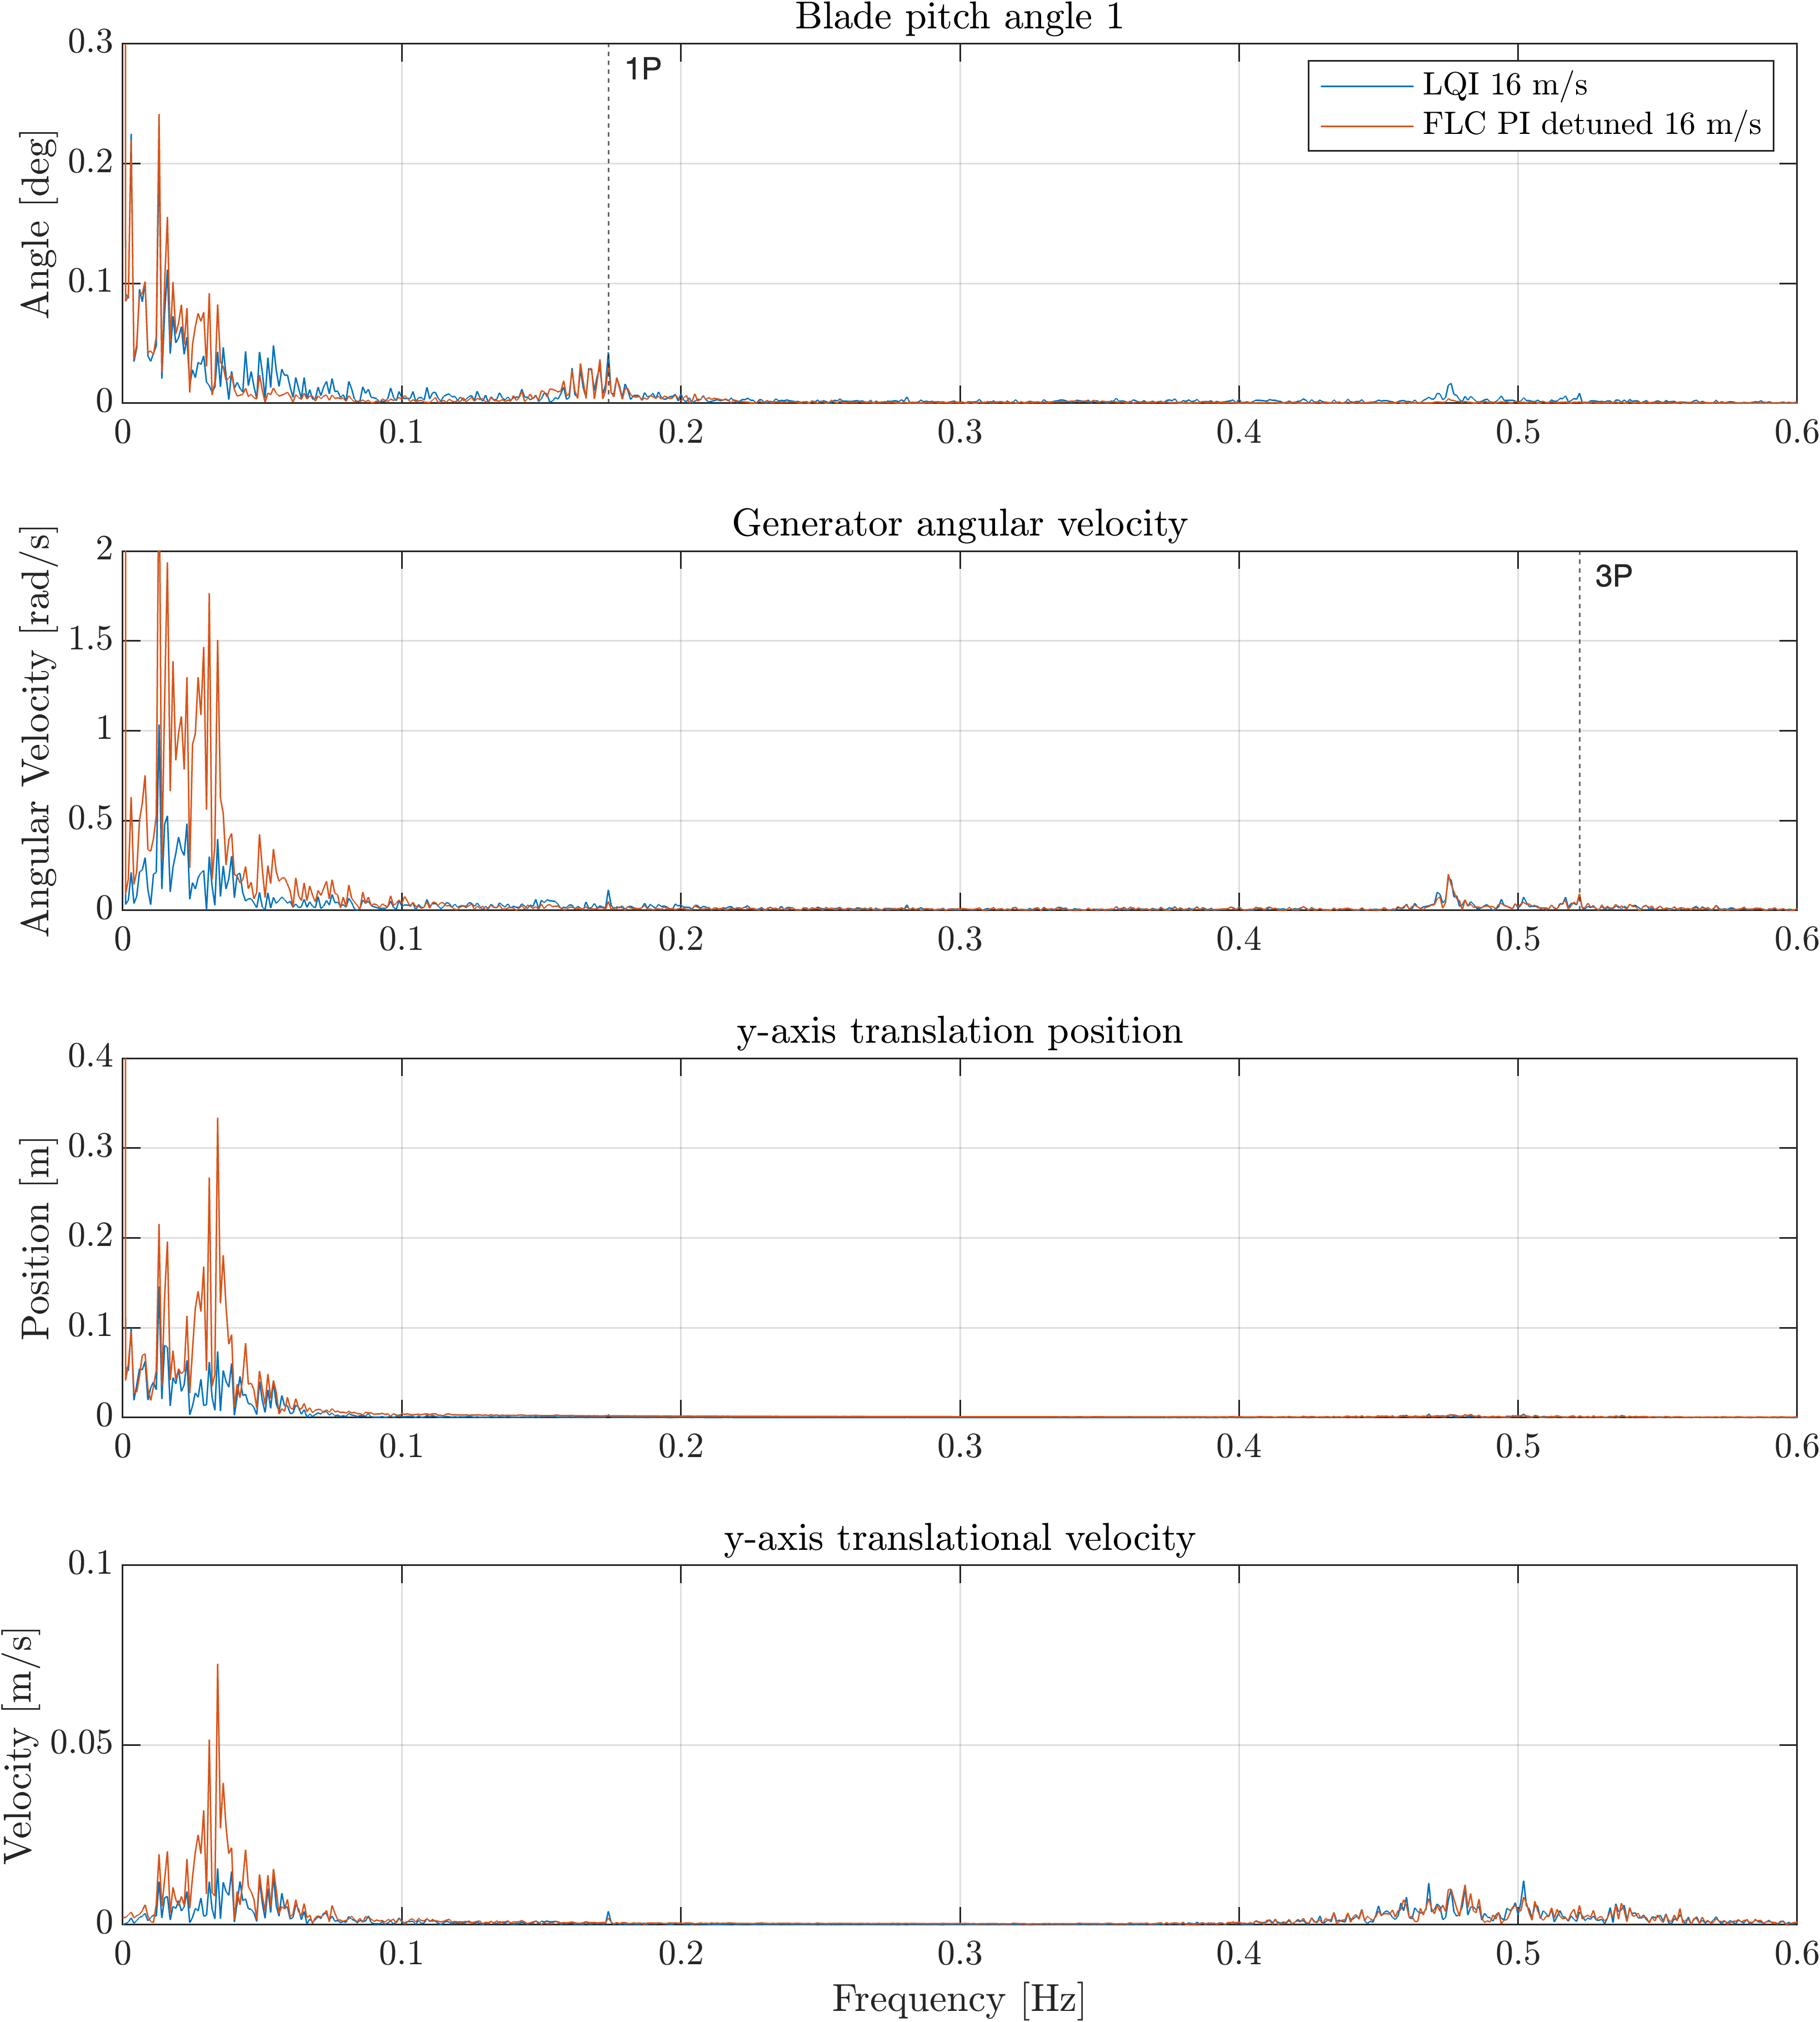
\includegraphics[width=0.7\linewidth]{Graphics/TestResults/VTSplotting/11_fft_th_w_py_vy.png}
	\caption{VTS simulation results.}
	\label{fig:vts_11_fft_th_w_py_vy}
\end{figure}

\begin{figure}[ht]
	\centering
	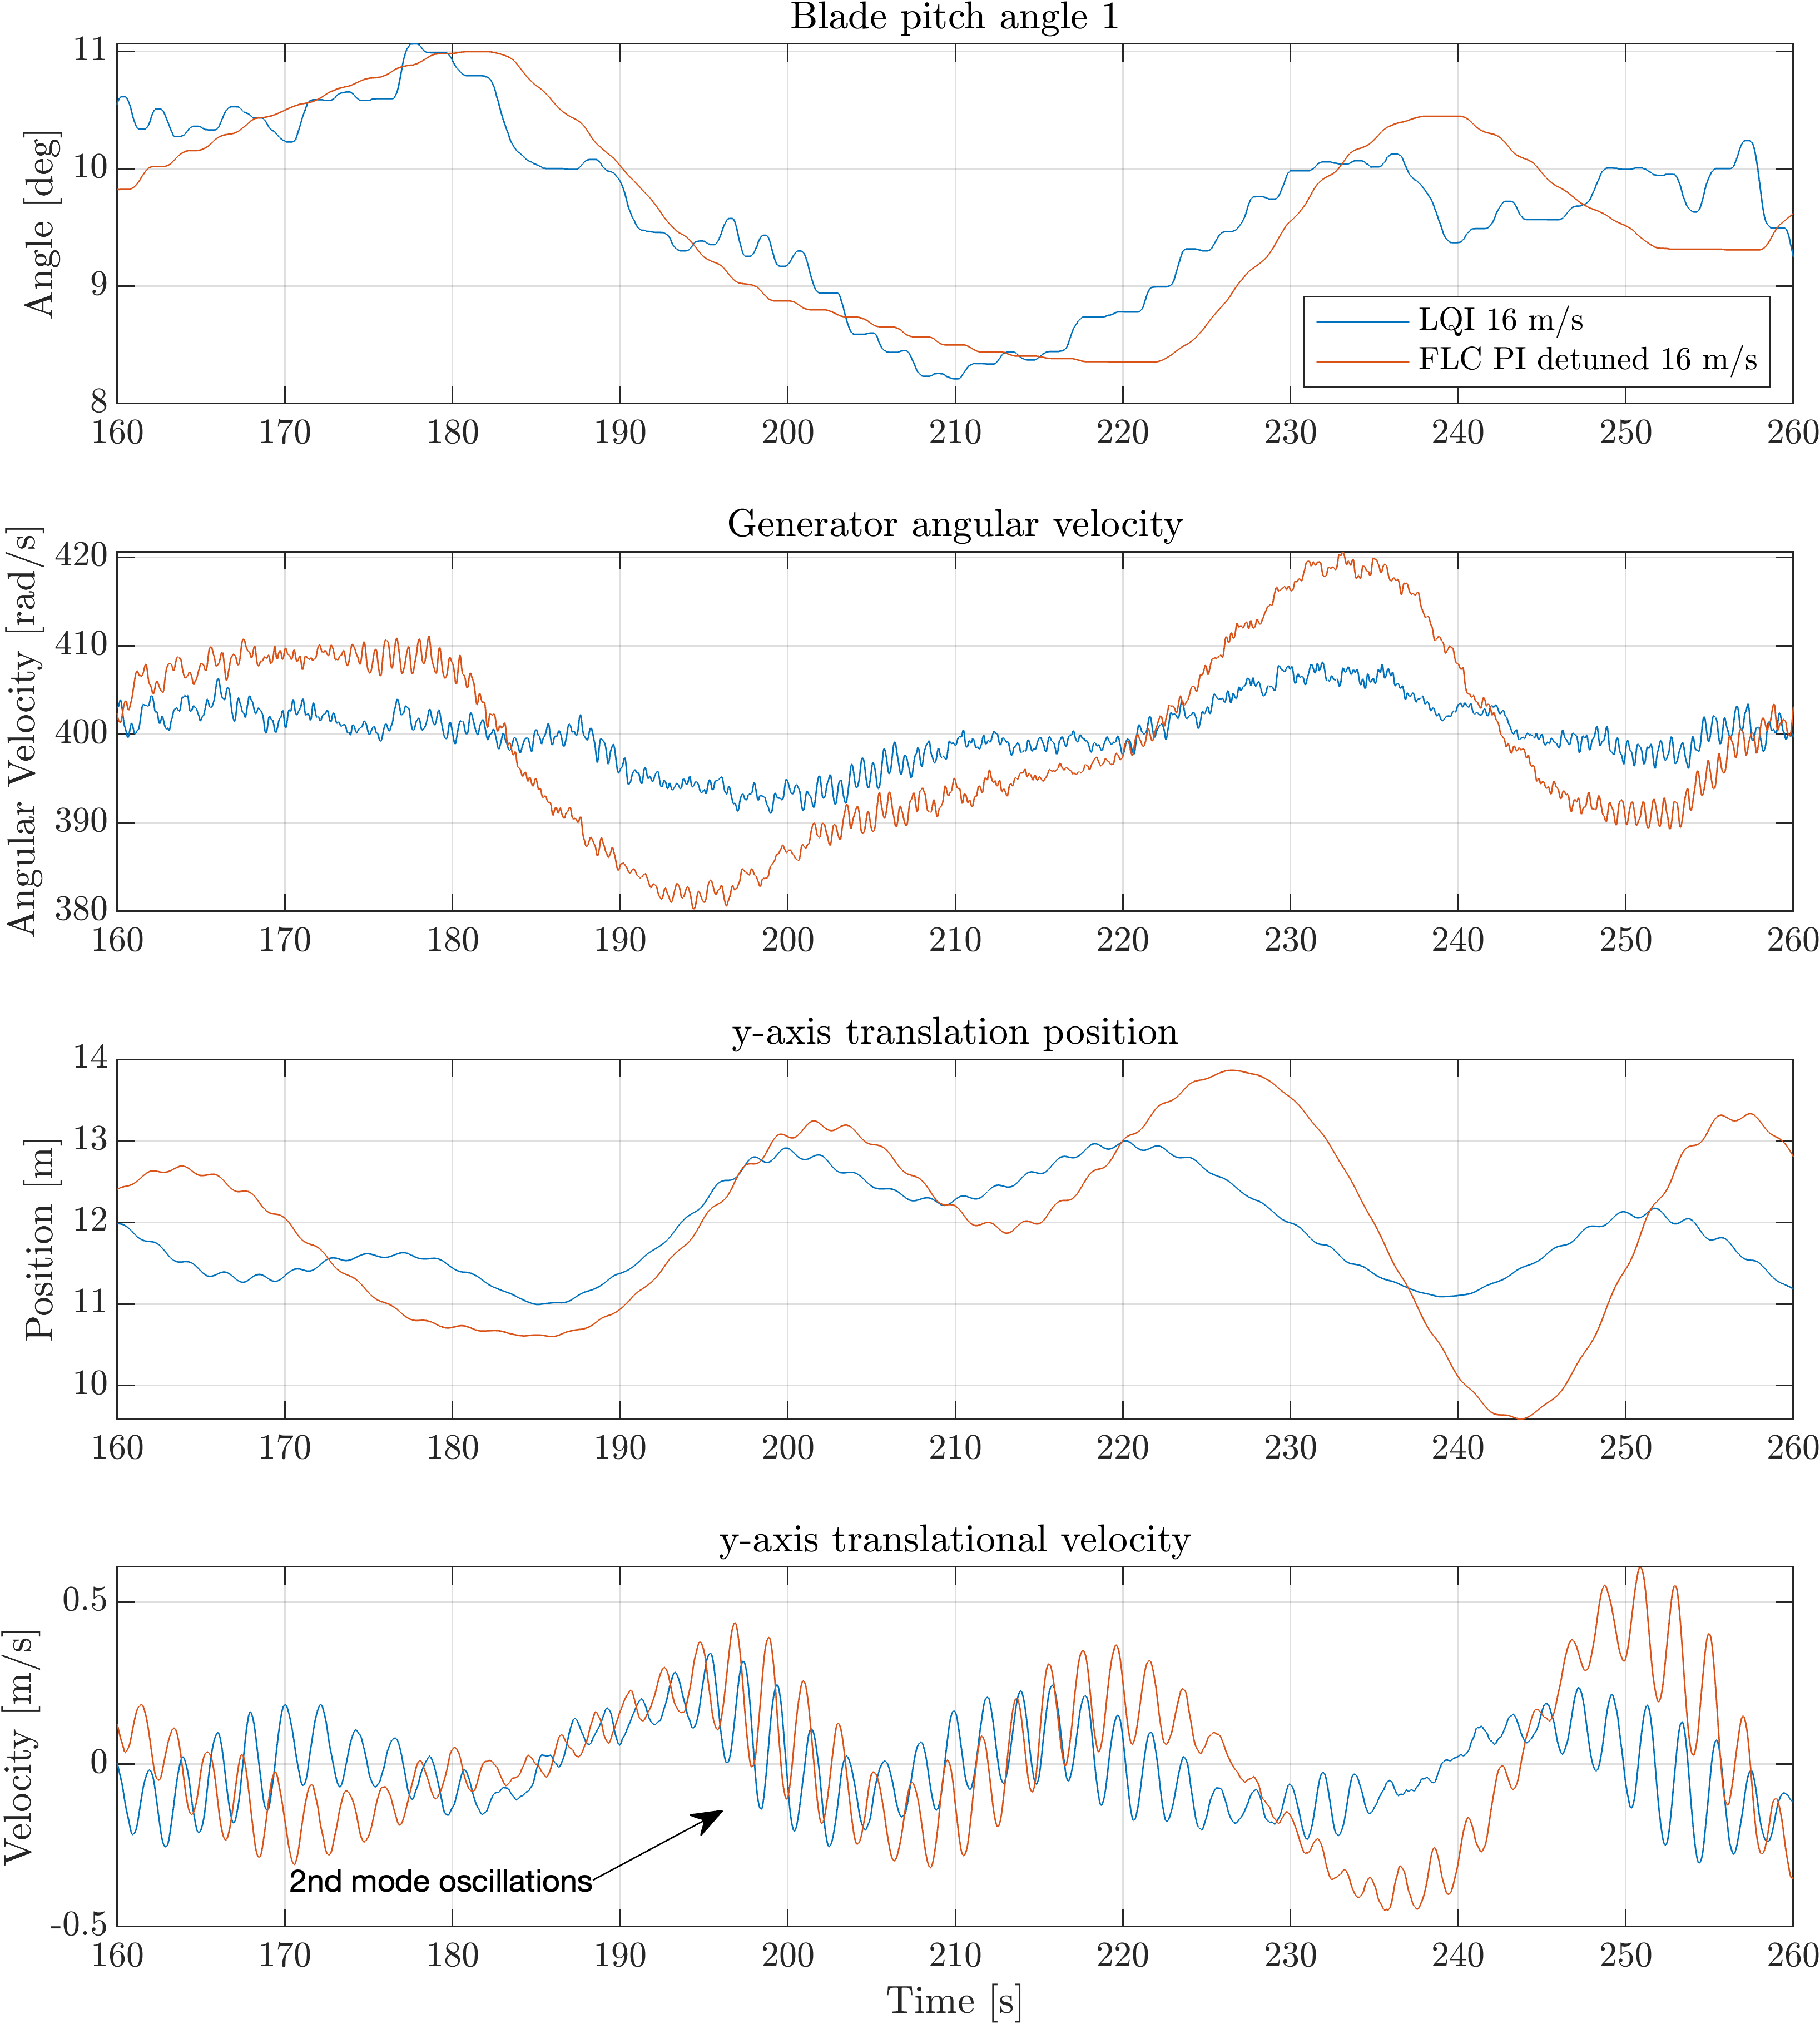
\includegraphics[width=0.7\linewidth]{Graphics/TestResults/VTSplotting/12_zoom_th_w_py_vy.png}
	\caption{VTS simulation results.}
	\label{fig:vts_12_zoom_th_w_py_vy}
\end{figure}

\begin{figure}[ht]
	\centering
	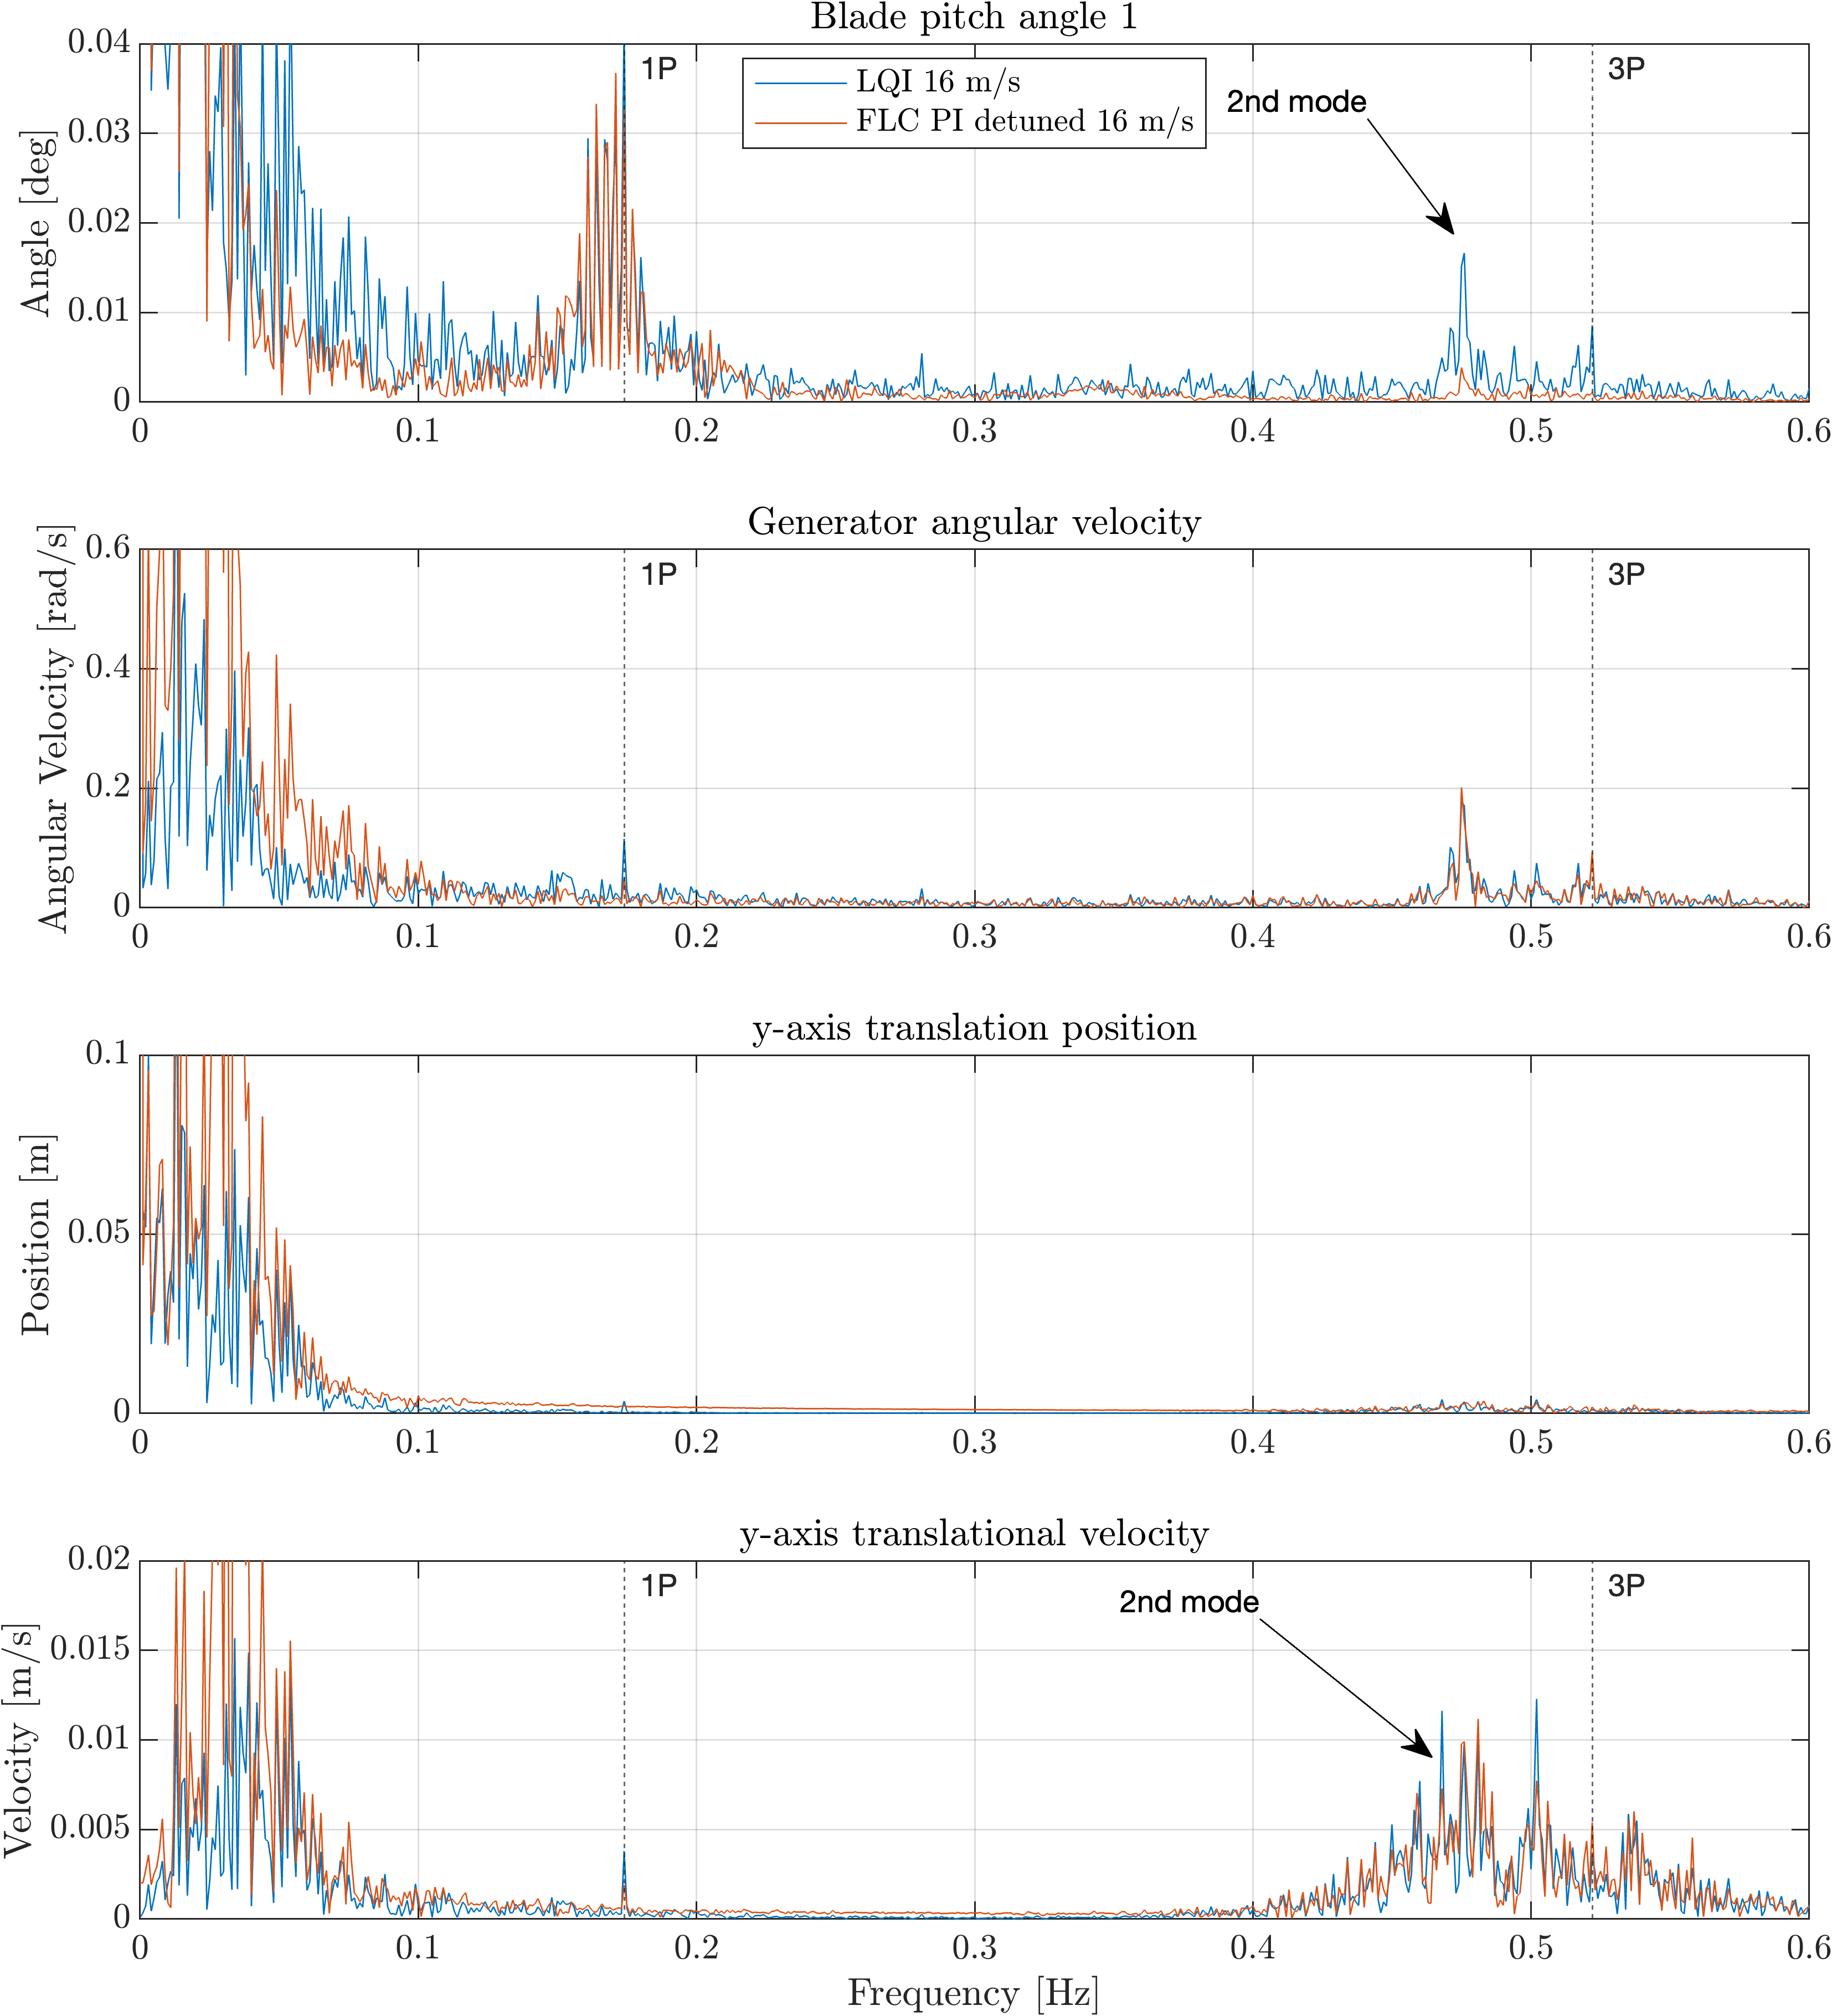
\includegraphics[width=0.7\linewidth]{Graphics/TestResults/VTSplotting/13_zoom_fft_th_w_py_vy.png}
	\caption{VTS simulation results.}
	\label{fig:vts_13_zoom_fft_th_w_py_vy}
\end{figure}

\subsection{Part 2}
Due to the increased rotor thrust sensitivity around nominal wind which is observed in \cref{fig:thrust_vs_windspeed} greater instability is expected for the 12 m/s simulations. The WT controller will furthermore change between PLC and FLC as the wind speed observed by the rotor goes above and below the nominal wind speed. This is expected to increase stability and worsen overall performance as well. At higher wind the rotor thrust sensitivity decreases and thus greater general stability and better performance is expected at 26 m/s.